\documentclass[12pt]{article}
\usepackage[margin=1in]{geometry}
\usepackage[utf8]{inputenc}
\usepackage{lmodern}
\usepackage{fancyhdr}
\usepackage{hyperref}
\usepackage[dvipsnames]{xcolor}
\usepackage{soul}
\usepackage{graphicx}
\usepackage{fancyvrb}
\usepackage[toc,title]{appendix}
\usepackage{titlesec}

\titleformat*{\section}{\LARGE\bfseries}
\titleformat*{\subsection}{\Large\bfseries}
\titleformat*{\subsubsection}{\large\bfseries}
\titleformat*{\paragraph}{\bfseries}
\titleformat*{\subparagraph}{\bfseries}

\titlespacing*{\section}{0pt}{0.5\baselineskip}{0.25\baselineskip}
\titlespacing*{\subsection}{0pt}{0.5\baselineskip}{0.25\baselineskip}
\titlespacing*{\subsubsection}{0pt}{0.5\baselineskip}{0.25\baselineskip}
\titlespacing*{\paragraph}{0pt}{0.5\baselineskip}{0.25\baselineskip}
\titlespacing*{\subparagraph}{0pt}{0.5\baselineskip}{0.25\baselineskip}

\renewcommand{\familydefault}{\sfdefault}

\pagestyle{fancy}
\fancyhf{}
\rhead{\thepage}
\lhead{STELLARIS SANDBOX: DML AND DDL QUERIES}
\renewcommand{\headrulewidth}{0pt}
\setlength{\headheight}{15pt}

\setlength{\parindent}{0em}
\setlength{\parskip}{1em}

\renewcommand\labelitemii{\textopenbullet}

\setcounter{secnumdepth}{4}

\newcommand{\hparagraph}[1]{\paragraph{#1}\mbox{}\vspace{0.75em}\\}
\newcommand{\hiparagraph}[1]{\paragraph{#1}\mbox{}\vspace{-2em}\\}

\definecolor{ResponseRed}{rgb}{0.917, 0.6, 0.6}
\DeclareRobustCommand{\fix}[1]{{\sethlcolor{YellowGreen}\hl{Fix:} #1}}
\DeclareRobustCommand{\response}[1]{{\sethlcolor{ResponseRed}\hl{Response:} #1}}

\begin{document}

\begin{titlepage}
    \vspace*{15em}{\centering\Huge Stellaris Sandbox: \\ Implement CREATE + READ operations\par}
    \vspace{1em}
    \centering \Large Matthew S. Macovsky \\
    \vspace{0.5em}
    \centering \Large Logan P. Traffas \\
    \vspace{1em}
    \centering \Large CS 340-400 Winter 2021 \\
    \vspace{1em}
    \centering \Large Oregon State University \\
    \vspace*{\fill}
    \large Link to HTML Interface: \url{http://flip3.engr.oregonstate.edu:3845/}
\end{titlepage}

\tableofcontents

\newpage
\section{Project Outline}

In the videogame Stellaris, players control galactic empires competing for control of a galaxy and its resources. Stellaris Sandbox is a database-driven website that will allow users to design a galaxy so that a game of Stellaris can be played in it. This will provide users with the freedom to create new starting circumstances for players, lending itself especially to role-playing oriented players. Stellaris has an average of 14,000 concurrent players on PC alone and a number of active online communities, together making up a large audience with a potential interest in the tool. A custom mod would be needed in order to import the galaxies designed in Stellaris Sandbox into the game itself. 

Using Stellaris Sandbox, users can create between 200 and 1000 Systems within the galaxy as well as the hyperlanes that connect them. Users can also create between 0 and 10 Bodies, such as planets, within Systems that can each contain 0 to 3 exploitable Resource deposits. AI-controlled Empires can also be created that span Systems and start off with given quantities of each Resource.

In Stellaris, there is only one galaxy, so Stellaris Sandbox will only allow design of a single galaxy at a time. Since users will be expected to create galaxies with a large number of Systems, Stellaris Sandbox will provide templates and other tools to automatically generate features which can then be edited by the user.

\newpage
\section{Database Outline}

\begin{itemize}
    \item Empires: Pre-existing, AI-controlled galactic empires
    \begin{itemize}
        \item empireID: int, auto\_increment, unique, not NULL, PK
        \item name: varchar(255), not NULL
        \item aggressiveness: varchar(16), not NULL, one of \{“passive”, “moderate”, “aggressive”\}
        \item primaryColor: varchar(7), not NULL, the color Hex code
        \item secondaryColor: varchar(7), not NULL, the color Hex code
        \item isFallenEmpire: bool, not NULL
        \item Relationship: 1:M between Empires and Systems, implemented with empireID as a FK within Systems. This relationship represents which empire owns the system.
        \item Relationship: M:M between Empires and Resources, implemented in a separate table with empireID and resourceID as FKs and an int resourceQuantity. This represents resource stockpiles owned by an empire. \hl{Logan Traffas will work  on this relationship in the database.}
        \item \hl{Matthew Macovsky will work on this \& the associated website aspects.}
    \end{itemize}
    \item Systems: Star systems connected by hyperlanes and controlled by empires
    \begin{itemize}
        \item systemID: int, auto\_increment, unique, not NULL, PK
        \item name: varchar(255), not NULL
        \item type: varchar(16), not NULL, one of \{“unary”, “binary”, “trinary”\}
        \item orbitalRadius: float, not NULL, between 0.25 and 1.0
        \item theta: float, not NULL, between 0 and 360. The theta and orbitalRadius attributes together indicate the positions of Systems in the galaxy using polar coordinates.
        \item empireID: int, FK
        \item Relationship: M:M between Systems, implemented in a separate table with system1 and system2 as FKs. This relationship consists of the hyperlane connections between systems. Matthew Macovsky and Logan Traffas will work together on this relationship in the database. 
        \item Relationship: 1:M between Systems and Bodies, implemented with systemID as a FK within Bodies. \hl{Logan Traffas will work on this \& the associated website aspects.}
        \item Indirect Relationship: M:M between Systems and Bodies, since Systems contain Bodies which are in turn related to Resources. Does not require explicit implementation in the database.
    \end{itemize}
    \item Bodies: Astronomical bodies that reside in systems (namely planets and asteroids)
    \begin{itemize}
        \item bodyID: int, auto\_increment, unique, not NULL, PK
        \item name: varchar(255), not NULL
        \item type: varchar(16), not NULL, one of \{“planet”, “asteroid”\}
        \item orbitalRadius: float, not NULL, between 0.1 and 1.0
        \item theta: float, not NULL, between 0 and 360. The theta and orbitalRadius attributes together indicate the positions of Bodies in Systems using polar coordinates.
        \item systemID: int, not NULL, FK
        \item Relationship: M:M between Bodies and Resources, implemented in a separate table with bodyID and resourceID as FKs and an int resourceQuantity. This represents resource deposits on a body that can produce that many of that resource per month. \hl{Matthew Macovsky will work on this relationship in the database.}
        \item \hl{Logan Traffas will work on this \& the associated website aspects.}
    \end{itemize}
    \item Resources: Resource deposits on bodies that can be exploited by empires
    \begin{itemize}
        \item resourceID: int, auto\_increment, unique, not NULL, PK
        \item name: varchar(255), not NULL
        \item baseMarketValue: float, greater than 0
        \item color: varchar(7), not NULL, the color Hex code
        \item \hl{Matthew Macovsky will work on this \& the associated website aspects.}
    \end{itemize}
\end{itemize}

\newpage
\section{Entity-Relationship Diagram}

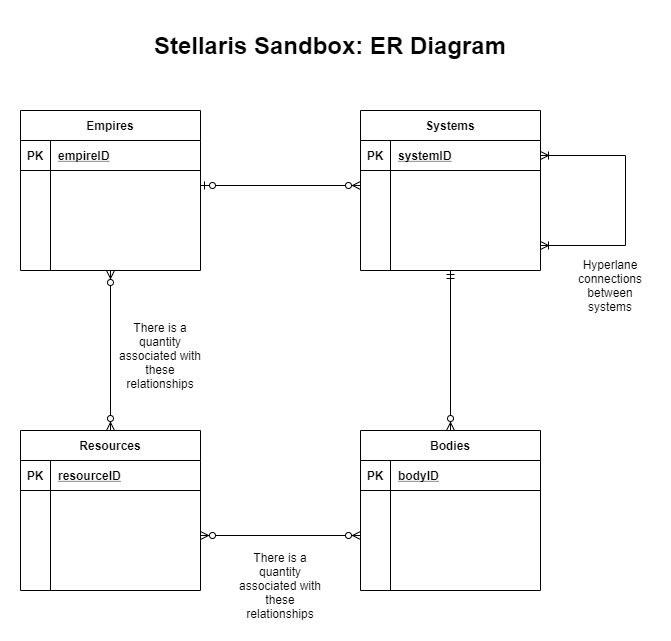
\includegraphics[width=\textwidth]{erd.png}

\newpage
\section{Schema}
\begin{small}
\begin{Verbatim}[commandchars=+\[\]]
Empires(
	+underline[empireID],
	name,
	aggressiveness,
	primaryColor,
	secondaryColor,
	isFallenEmpire)

Systems(
	+underline[systemID],
	name,
	type,
	orbitalRadius,
	theta,
	empireID)

Bodies(
	+underline[bodyID],
	name,
	type,
	orbitalRadius,
	theta,
	systemID)

Resources(
	+underline[resourceID],
	name,
	baseMarketValue,
	color)

Hyperlanes(
	+underline[system1ID],
	+underline[system2ID])
	
ResourceStock(
	+underline[empireID],
	+underline[resourceID],
	quantity)

ResourceDeposits(
	+underline[bodyID],
	+underline[resourceID],
	quantity)
\end{Verbatim}
\end{small}

\newpage

\begin{appendices}
\section{Upgrades to Draft}

\subsection{Step 2}
None.

\subsection{Step 3 Draft}
\begin{itemize}
    \item Change colors to use RGB hex color codes rather than a choice between a small number of colors.
\end{itemize}

\subsection{Step 3}
None.

\subsection{Step 4}
\begin{itemize}
    \item Replaced the Systems int starCount attribute with a varchar(16) type attribute that can be one of \{“unary”, “binary”, “trinary”\}. Because of the few options available, it makes more sense and is more immersive to use these names rather than a number.
    \item Changed color attributes to be varchar(7) instead of varchar(6) so that they could include the \# symbol in the hex code color (ex: \#FFFFFF)
\end{itemize}

\subsection{Step 5}
\begin{itemize}
    \item Change minimum system orbitalRadius to 0.25 in the outline.
\end{itemize}

\newpage
\section{Feedback and Fixes}

\subsection{Grader Feedback (Step 1)}
\subsubsection{Maximum text length not specified}
\hparagraph{Feedback}
“text should be \texttt{varchar(<max\_length\_of\_text>)} e.g.\texttt{varchar(255)}”
\hparagraph{Fix/Response}
Specify text attributes as \texttt{varchar(max\_text\_length)}.

\subsubsection{Lack of foreign key attributes}
\hparagraph{Feedback}
“You specify that there is a 1:M relationship between Empires and Systems with empireID acting as the FK in Systems, but there is no empireID attribute in Systems. Same issue with Systems and Bodies.”
\hparagraph{Fix/Response}
Add FKs to Bodies and Systems to enable 1:M relationships.

\subsubsection{Lack of clarity in relationship meaning}
\hparagraph{Feedback}
“The M:M relationship between Systems and Systems is fine, but please clarify that the relationship indicates the hyperlane connections between the two (which is what I inferred).”
\hparagraph{Fix/Response}
Clarify that the M:M relationships between Systems and Systems represent hyperlanes between the related systems.

\newpage
\subsection{Draft Review (Step 2)}
\subsubsection{Review 1}
\hiparagraph{Contents}
\begin{itemize}
    \item \textbf{Does the overview describe what problem is to be solved by a website with DB back end?}
    \begin{itemize}
        \item I think a little more clarity here could help. The overview explicitly states that people can create galaxies for the video game that I gather will then be ported to the game itself so people can play within the galaxy. I'm guessing the problem to be solved is that creating galaxies is time consuming and there is a creative aspect that lends itself well to being open to creators who can help the game designers come up with original and unique galaxies to play within. The 'why' that I'm guessing here isn't explicitly stated.
    \end{itemize}
    \item \textbf{Does the overview list specific facts?}
    \begin{itemize}
        \item No. I'm not sure how many people they expect to play this game or the benefits of opening up galaxy creation to the public. I get the idea but no context was given as to the why.
    \end{itemize}
    \item \textbf{Are at least four entities described and does each one represent a single idea to be stored as a list?}
    \begin{itemize}
        \item Yes.
        \item I noticed the Schema has two additional tables(?) that are not present on the ERD.
    \end{itemize}
    \item \textbf{Does the outline of entity details describe the purpose of each, list attribute datatypes and constraints and describe relationships between entities?  Does the outline clearly indicate which entities (tables) will be implemented and which team member is primarily assigned to the associated page(s)?}
    \begin{itemize}
        \item Yes: Purpose of each
        \item Yes: List attribute datatypes and constraints
        \item Yes: Describe relationship between entities
        \item No: Which team member is primarily assigned to the associated pages
    \end{itemize}
    \item \textbf{Are 1:M relationships correctly formulated? Is there at least  one M:M relationship?}
    \begin{itemize}
        \item Yes, correctly formulated and at least one M:M
    \end{itemize}
    \item \textbf{Is there consistency in a) naming between overview and entity/attributes b) entities plural, attributes singular c) use of capitalization for naming?}
    \begin{itemize}
        \item Yes, consistency present.
    \end{itemize}
\end{itemize}
\hiparagraph{Fixes/Responses}
\begin{itemize}
    \item \fix{Clarify purpose and audience of tool in project overview.}
    \item \fix{Add player numbers to project overview.}
    \item \response{The tables not present in the ERD are M:M relationship tables. No fix needed.}
    \item \fix{Assign team members to entities.}
\end{itemize}

\subsubsection{Review 2}
\hiparagraph{Contents}
\begin{itemize}
    \item \textbf{Does the overview describe what problem is to be solved by a website with DB back end?}
    \begin{itemize}
        \item It seems like it may be a companion for a tabletop rpg, similar to D\&D, or a computer game like Minecraft, where someone can setup a world/server and invite others to join. This will allow someone to setup the star system in their universe so that the game can then be played. After reading through it again it kind of seems like a mix of the games Civilization and No Mans Sky.
    \end{itemize}
    \item \textbf{Does the overview list specific facts?}
    \begin{itemize}
        \item It lists facts about the number of different things that can be implemented but not about number of users. Seems like it can be 1 to many users since it mentions AI empires can be generated.
    \end{itemize}
    \item \textbf{Are at least four entities described and does each one represent a single idea to be stored as a list?}
    \begin{itemize}
        \item Yes, there are 4 entities.
    \end{itemize}
    \item \textbf{Does the outline of entity details describe the purpose of each, list attribute data types and constraints and describe relationships between entities?  Does the outline clearly indicate which entities (tables) will be implemented and which team member is primarily assigned to the associated page(s)?}
    \begin{itemize}
        \item The outline lists the entities along with attributes and their types. A bit of description would be helpful for people unfamiliar with them. For instance, Theta is an attribute in a few tables ranging from 0 - 360 (degrees). I am guessing that it is probably the location of the object in its orbit gut it could also be associated with the spin or tilt of the object as well. The tables that are mentioned for containing the M:M relationships are not in the outline or ER diagram.
    \end{itemize}
    \item \textbf{Are 1:M relationships correctly formulated? Is there at least  one M:M relationship?}
    \begin{itemize}
        \item It seems like they are correctly formatted based on the ER diagram. The schema doesn't list what are foreign keys and would be easier to see if it was in a diagram with arrows going from entities to foreign keys. There is more than 1 M:M relationship.
    \end{itemize}
    \item \textbf{Is there consistency in a) naming between overview and entity/attributes b) entities plural, attributes singular c) use of capitalization for naming?}
    \begin{itemize}
        \item Yes, everything seems to be consistent with naming, plurality, and case.
    \end{itemize}
\end{itemize}
\hiparagraph{Fixes/Responses}
\begin{itemize}
    \item \fix{Clarify what theta is.}
    \item \response{The ER diagram is only required to have primary keys listed.}
\end{itemize}

\subsubsection{Review 3}
\hiparagraph{Contents}
\begin{itemize}
    \item \textbf{Does the overview describe what problem is to be solved by a website with DB back end?}
    \begin{itemize}
        \item The overview clearly spells out your goals. I am wondering whether an empire could relate to systems across multiple galaxies or if it would be limited to systems a single galaxy. Similarly, I wonder if hyperplanes can connect systems across galaxies or if they would be limited to making connections within a single galaxy.
    \end{itemize}
    \item \textbf{Does the overview list specific facts?}
    \begin{itemize}
        \item Yes, the numerical specificity and clarity of the relationships (with the exceptions identified above) is good. I wonder about implementing the minimum bound of 200 systems per galaxy. This makes sense to me conceptually, but I think it could be painful from the perspective of a user needing to create 200 systems in order to initialize a galaxy.
    \end{itemize}
    \item \textbf{Are at least four entities described and does each one represent a single idea to be stored as a list?}
    \begin{itemize}
        \item Yes
    \end{itemize}
    \item \textbf{Does the outline of entity details describe the purpose of each, list attribute datatypes and constraints and describe relationships between entities?  Does the outline clearly indicate which entities (tables) will be implemented and which team member is primarily assigned to the associated page(s)?}
    \begin{itemize}
        \item Yes, great job
    \end{itemize}
    \item \textbf{Are 1:M relationships correctly formulated? Is there at least  one M:M relationship?}
    \begin{itemize}
        \item The M:M empire\_resources relationship doesn't make sense to me in context of the hierarchical design described in your overview. For example, if an empire owns a system, which contains bodies, which contain resources, doesn't that empire already own the resources by extension? Wouldn't a separate empire\_resources linking table either duplicate that ownership or indicate conflicting ownership?
        \item In describing the 1:M relationship between systems and bodies, you have written: "This relationship consists of the hyperlane connections between systems. I think maybe that statement belongs in the description of the M:M system to system relationship.
        \item it seems to me that the resourceQuantity attribute should be assigned to the Resources table, not the M:M relationship between bodies and resources. Here I'm assuming that if resources are collected from a resource, all associated systems should see that change. The M:M relationship between resources and systems also seems inconsistent to me with your overview which indicates resources are "contained" in systems. Please see my first comment in response to this question, as I think that issue is tied into this as well. I think the broader conceptual question needing clarification is: what is the conceptual nature of a resource and how a resource is shared (e.g. can two bodies in the same system share a resource? can two bodies in separate systems share a resource? two bodies in separate galaxies?)?
    \end{itemize}
    \item \textbf{Is there consistency in a) naming between overview and entity/attributes b) entities plural, attributes singular c) use of capitalization for naming?}
    \begin{itemize}
        \item Yes, this looks good to me, though it might make things easier to use plural or singular in both the table names and the key names (both foreign and primary) e.g. Empire and empireID or Empires and empiresID. I just just think it's possible this would make writing queries easier.
    \end{itemize}
\end{itemize}
\hiparagraph{Fixes/Responses}
\begin{itemize}
    \item \fix{Clarify that Stellaris only allows for a single galaxy.}
    \item \fix{Add that tool will have the capability to randomly generate systems.}
    \item \fix{Clarify that empires have planets which contain exploitable resource deposits (x resources/month) as well as their own stockpiles of resources.}
    \item \fix{Move clarification about hyperlanes to correct relationship description.}
    \item \response{There is no relationship between systems and resources.}
    \item \response{We prefer the table names to be plural (as they will contain many entities) and the attribute names to be singular (as they will contain the ID of a single entity).}
\end{itemize}

\subsubsection{Review 4}
\hiparagraph{Contents}
\begin{itemize}
    \item \textbf{Does the overview describe what problem is to be solved by a website with DB back end?}
    \begin{itemize}
        \item The database will be in charge of maintaining newly created systems, bodies, and resources, as well as tracking changes over time that happen between the systems.
    \end{itemize}
    \item \textbf{Does the overview list specific facts?}
    \begin{itemize}
        \item Yes, they do a good job of being thorough with each attribute. I also think it was smart that they limited the systems, bodies, and resources to the numbers they chose. With what they are trying to achieve those seem like well thought out parameters.
    \end{itemize}
    \item \textbf{Are at least four entities described and does each one represent a single idea to be stored as a list?}
    \begin{itemize}
        \item Yes. I'm a bit confused on some of these entities which I explain in the next part.
    \end{itemize}
    \item \textbf{Does the outline of entity details describe the purpose of each, list attribute datatypes and constraints and describe relationships between entities?  Does the outline clearly indicate which entities (tables) will be implemented and which team member is primarily assigned to the associated page(s)?}
    \begin{itemize}
        \item For the second question, they list out tasks well and seem spread out effectively.
        \item You list that Empires to Systems will be 1 to M but the ERD shows M:M
        \item I'm a bit confused on the Systems Entity. Are Star Systems being treated like cities, where say Portland (Star System) is in Oregon (Empire), and that theoretically we could go from one city to another, one star system to another star system.
        \item I'm a bit confused on the relationship from Empires to Systems, which says there must be at least one system to a empire. What happens to the system attached to the empire when it falls? If an empire can fall, it seems like it should be 0 | to all the connected pieces.
        \item Are asteroids always orbiting something since there must be an orbitalRadius?
    \end{itemize}
    \item \textbf{Are 1:M relationships correctly formulated? Is there at least  one M:M relationship?}
    \begin{itemize}
        \item Shouldn't there be another table for the M:M from Empires to Systems? 
        \item The other 1:M relationships seem fine.
    \end{itemize}
    \item \textbf{Is there consistency in a) naming between overview and entity/attributes b) entities plural, attributes singular c) use of capitalization for naming?}
    \begin{itemize}
        \item Yes, in response to the review above, I think that have the key names be singular helps to solidify these are individual parts of the entity. Having everything be plural confuses me.
        \item I'm a fan of camelCase
    \end{itemize}
\end{itemize}
\hiparagraph{Fixes/Responses}
\begin{itemize}
    \item \fix{Correct the relationship in the ERD between Empires and Systems to be 1:M.}
    \item \response{Ships can move between star systems, but that isn’t part of this tool, only part of the game itself. Empires can claim ownership of star systems in their entirety.}
    \item \response{This is a valid point during gameplay, but since the tool is for designing starting galaxies no empire will be without a system.}
    \item \response{In Stellaris, asteroids, like planets, always orbit the system’s star(s).}
    \item \response{The M:M relationship between Empires and Systems in the ERD was an error.}
    \item \response{See response to the point about pluralization in the previous review.}
\end{itemize}

\newpage
\subsection{Grader Feedback (Step 3 Draft)}
\subsubsection{Lack of clarity in relationship between Systems and Resources}
\hparagraph{Feedback}
“I'm iffy on the argument that there are no relationships between systems and resources. There is because a system has a body and a body has resources. So its an indirect 1:M relationship. I'm not going to say you have to make any changes other than maybe expand, perhaps in your overview what the relationship is between Systems > Bodies > Resources and explicitly state why Systems has no relationship with Resources.”
\hparagraph{Fix/Response}
\fix{Add clarification in section about the Systems entity that there is an indirect M:M relationship between Systems and Resources via the relationship between Systems and Bodies.}

\newpage
\subsection{Draft Review (Step 3)}
\subsubsection{Review 1}
\hparagraph{Contents}
Matthew and Logan, it looks like you have a good start on your project. You have created a cool looking interface so far. I saw the tables for Resources and Bodies, but the pages for Empires and Systems were not loading, so I'm guessing these still might be in progress. I noticed you had the ability to add rows for both Resources and Bodies, but are still working on update and delete functionality. I also didn't see anything representing the relationships, so maybe these are coming when Empires and Systems are added as well.
\hiparagraph{Fixes/Responses}
\begin{itemize}
    \item \response{The Empires and Systems pages loaded correctly when tried by both of us - we’re not sure what the issue the reviewer had was.}
    \item \fix{Create the missing relationship management pages for Hyperlanes, ResourceStock, and ResourceDeposits.}
\end{itemize}

\subsection{Grader Feedback (Step 3)}
\subsubsection{Missing pages for relationships}
\hparagraph{Feedback}
“Just make sure you don't forget to represent your Hyperlanes, ResourceStock and ResourceDeposits on the web app. I did not see anywhere they were represented.”
\hparagraph{Fix/Response}
\fix{Create the missing relationship management pages for Hyperlanes, ResourceStock, and ResourceDeposits.}

\newpage

\subsection{Draft Review (Step 4)}

\subsubsection{Review 1}
\hparagraph{Contents}
\textbf{Data Manipulation Queries:}
\begin{itemize}
    \item \textbf{Are the queries syntactically correct? Disregard the part where input will be substituted as shown in the sample\_data\_manipulation\_queries.sql}
    \begin{itemize}
        \item Upon inspection of the data manipulation query file the queries do look syntactically correct.
    \end{itemize}
    \item \textbf{Are there queries providing all functionalities as required by the CS340 Project Guide ? What query is missing ? What needs to be fixed?}
    \begin{itemize}
        \item Yes the queries do provide all required functionalities and reflect CRUD. I can’t see anything that needs to be fixed.
    \end{itemize}
    \item \textbf{Do the queries cover the relationships as required by the CS340 Project Guide?}
    \begin{itemize}
        \item The queries do appear to cover the four required relationships for final implementation which include at least 1 many to many relationship.
    \end{itemize}
\end{itemize}
\textbf{DDQ File:}
\begin{itemize}
    \item \textbf{Is the SQL file syntactically correct? This can be easily verified by importing/copy-pasting it in phpmyadmin. (Do not forget to take backup of your own database before you do this!)}
    \begin{itemize}
        \item The SQL file is syntactically correct. Uploading the file took some time to process maybe due to the file size. However upon refreshing the bodies, empires, hyperlanes, resources, resource\_deposits, resource\_stocks, and systems appeared to upload with all their relevant data. However, upon submitting the file again I had the following static error:
        
        \texttt{3 errors were found during analysis.
            \\ \\
            1. A symbol name was expected! A reserved keyword can not be used as a column name without backquotes. (near "CHECK" at position 283) \\
            2. Unexpected beginning of statement. (near "primaryColor" at position 290) \\
            3. Unrecognized statement type. (near "RLIKE" at position 303) \\
            \#1050 - Table 'empires' already exists}
    \end{itemize}
    \item \textbf{Are the data types appropriate considering the description of the attribute in the database outline?}
    \begin{itemize}
        \item Yes, the data types are appropriate considering the database outline’s description of the table attributes.
    \end{itemize}
    \item \textbf{Are the foreign keys correctly defined when compared to the Schema?}
    \begin{itemize}
        \item The foreign keys do appear to be correctly defined when referning the database outline schema in the pdf submission against the info on my database form the sql file.
    \end{itemize}
    \item \textbf{Are relationship tables present when compared to the ERD/Schema?}
    \begin{itemize}
        \item Yes the relationship tables are present when compared to the ERD/Schema such as the resource\_deposits, resource\_stocks, and hyperlanes.
    \end{itemize}
\end{itemize}
\hiparagraph{Fixes/Responses}
\begin{itemize}
    \item \response{We haven't experienced any errors running our data definition file, and it doesn't seem like any of the other reviewers did either, so we're not sure what happened for this reviewer. We suspect it has to do with loading the queries twice as we don't delete any of the tables in our data definition file.}
\end{itemize}

\newpage
\subsubsection{Review 2}
\hparagraph{Contents}
\textbf{DMQ}
\begin{itemize}
    \item \textbf{Are the queries syntactically correct?}
    \begin{itemize}
        \item Yes, most are straightforward, and I double checked that the hyperlane SELECT functions as intended. Good work.
    \end{itemize}
    \item \textbf{Are there queries providing all functionalities as required by the CS340 Project Guide ? What query is missing ? What needs to be fixed?}
    \begin{itemize}
        \item I believe you are missing an UPDATE query which will null out a 1:M relationship (2nd to last bullet point in Specifications under Project Guide). In your project, this could be achieved by editing your UPDATE query within the Individual Systems View to allow it to set empireID. A certain button on the website could call this UPDATE to set empireID to null, meaning the empire lost control of the system or something. Otherwise, everything looks great.
    \end{itemize}
    \item \textbf{Do the queries cover the relationships as required by the CS340 Project Guide?}
    \begin{itemize}
        \item Yes, other than the null UPDATE above.
    \end{itemize}
\end{itemize}
\textbf{DDQ}
\begin{itemize}
    \item \textbf{Is the SQL file syntactically correct? This can be easily verified by importing/copy-pasting it in phpmyadmin. (Do not forget to take backup of your own database before you do this!)}
    \begin{itemize}
        \item It took a while o upload but everything checks out.
    \end{itemize}
    \item \textbf{Are the data types appropriate considering the description of the attribute in the database outline?}
    \begin{itemize}
        \item You were pretty particular about setting validation constraints on all your attributes. I did notice that your theta and orbital radius are not limited to the ranges you specified in the outline. 
    \end{itemize}
    \item \textbf{Are the foreign keys correctly defined when compared to the Schema?}
    \begin{itemize}
        \item Yes, they're all present
    \end{itemize}
    \item \textbf{Are relationship tables present when compared to the ERD/Schema?}
    \begin{itemize}
        \item Yes, all three are present.
    \end{itemize}
\end{itemize}
Really clean implementation so far, keep it up.
\hiparagraph{Fixes/Responses}
\begin{itemize}
    \item \response{It is possible to do this already - there is a "None" option in the dropdown for a system's owning empire.}
    \item \fix{Add range constraints to theta and orbital radius in the data definition file to match the outline.}
\end{itemize}

\newpage
\subsubsection{Review 3}
\hparagraph{Contents}
\textbf{DMQ}
\begin{itemize}
    \item \textbf{Are the queries syntactically correct?}
    \begin{itemize}
        \item Yep, the queries appear to be syntactically correct according to the file.
    \end{itemize}
    \item \textbf{Are there queries providing all functionalities as required by the CS340 Project Guide ? What query is missing ? What needs to be fixed?}
    \begin{itemize}
        \item It appears as though all queries cover the required functionalities. The comment above mentions a missing UPDATE for 1:M relationship but I think this is taken care of in the UPDATE queries defined for the empire view.
    \end{itemize}
    \item \textbf{Do the queries cover the relationships as required by the CS340 Project Guide?}
    \begin{itemize}
        \item Yep! The required relationships are covered. 
    \end{itemize}
\end{itemize}
\textbf{DDQ}
\begin{itemize}
    \item \textbf{Is the SQL file syntactically correct? This can be easily verified by importing/copy-pasting it in phpmyadmin. (Do not forget to take backup of your own database before you do this!)}
    \begin{itemize}
        \item Yes, everything was imported correctly after a minute or so. 
    \end{itemize}
    \item \textbf{Are the data types appropriate considering the description of the attribute in the database outline?}
    \begin{itemize}
        \item Yes, data types seem appropriate.
    \end{itemize}
    \item \textbf{Are the foreign keys correctly defined when compared to the Schema?}
    \begin{itemize}
        \item All foreign keys are correctly defined.
    \end{itemize}
    \item \textbf{Are relationship tables present when compared to the ERD/Schema?}
    \begin{itemize}
        \item All relationships are present. 
    \end{itemize}
\end{itemize}
\hparagraph{Fixes/Responses}
None.

\newpage
\subsubsection{Review 4}
\hparagraph{Contents}
\textbf{Data Manipulation Queries:}
\begin{itemize}
    \item \textbf{Are the queries syntactically correct? Disregard the part where input will be substituted as shown in the sample\_data\_manipulation\_queries.sql}
    \begin{itemize}
        \item They are correct
    \end{itemize}
    \item \textbf{Are there queries providing all functionalities as required by the CS340 Project Guide ? What query is missing ? What needs to be fixed?}
    \begin{itemize}
        \item I don't see anything missing
    \end{itemize}
    \item \textbf{Do the queries cover the relationships as required by the CS340 Project Guide?}
    \begin{itemize}
        \item They do
    \end{itemize}
\end{itemize}
\textbf{DDQ File:}
\begin{itemize}
    \item \textbf{Is the SQL file syntactically correct? This can be easily verified by importing/copy-pasting it in phpmyadmin. (Do not forget to take backup of your own database before you do this!)}
    \begin{itemize}
        \item The SQL file is syntactically correct and no errors were found while uploading.
    \end{itemize}
    \item \textbf{Are the data types appropriate considering the description of the attribute in the database outline?}
    \begin{itemize}
        \item Yes, they are appropriate
    \end{itemize}
    \item \textbf{Are the foreign keys correctly defined when compared to the Schema?}
    \begin{itemize}
        \item Yes, the foreign keys are correct
    \end{itemize}
    \item \textbf{Are relationship tables present when compared to the ERD/Schema?}
    \begin{itemize}
        \item Yes they are all present
    \end{itemize}
\end{itemize}
\hparagraph{Fixes/Responses}
None.

\end{appendices}

\end{document}
